\documentclass{article}
 \usepackage[utf8]{inputenc}
 \usepackage{graphicx}
 \graphicspath{ {images/} }
 \begin{document}

 \title{ARTIFICIAL INTELLIGENCE EXAM}
 \author{Course Code: 1DL340}
 \date{Ref.  This is a student generated exam. }
 \maketitle

 This exam has  18  questions for a total of  49  marks. Grade boundaries are:

 \begin{center}
 3 -  24.5 

 4 -  32.5 

 5 -  40.5 

 \end{center}

 In exceptional circumstances these boundaries may be adjusted at the discretion of the examiner. This would be done on an exam-wide basis, NOT for individual students.

 You are permitted to make use of a calculator and language dictionary in this exam.
\clearpage
\section{A-Star}

Table~\ref{AStar_Edges} gives the edge values for a shortest path problem. Using these and the A* algorithm, find the shortest path from the start node to the goal node. Provide a valid heuristic and show all working. (4 marks)

\begin{table}[h!]
\caption{Edges}
\label{AStar_Edges}
\begin{center}
\begin{tabular}{ |c||c|c|c|c|c|c|c| } 
\hline
 & Start & A & B & C & D & E & Goal\\
\hline
Start & 0 & 5 & 4 & 0 & 0 & 0 & 0\\
A & 0 & 0 & 6 & 0 & 6 & 0 & 0\\
B & 0 & 0 & 0 & 7 & 0 & 0 & 0\\
C & 0 & 0 & 0 & 0 & 2 & 0 & 0\\
D & 0 & 0 & 0 & 0 & 0 & 7 & 0\\
E & 0 & 0 & 0 & 0 & 0 & 0 & 3\\
Goal & 0 & 0 & 0 & 0 & 0 & 0 & 0\\
\hline
\end{tabular}
\end{center}
\end{table}
\clearpage
\section{MCMC and Directed Graphical Models}

Tables~\ref{MCMC1} to~\ref{MCMC5} provide the conditional probability distributions for a directed graphical model.

A. Use this information to draw the graph of the associated directed graphical model. (1 mark)

B. Table~\ref{MCMC6} provides observed values for some of the nodes. Given these, the initial values provided in Table~\ref{MCMC7} and the random numbers provided below, use the Metropolis within Gibbs MCMC sampling algorithm to generate two complete samples of the variables. Assume that the candidate function gives the opposite of the current value. At each step, explain what value you are considering, what the current and candidate values are, and why you updated it or did not update it. (4 marks)

Random numbers: 0.839,0.753,0.534,0.923,0.72,0.739 
\begin{table}[h!]
\caption{P(A)}
\label{MCMC1}
\begin{center}
\begin{tabular}{ |c||c|c| } 
\hline
 - & A=F & A=T\\
\hline
 & 0.75 & 0.25\\
\hline
\end{tabular}
\end{center}
\end{table}
\begin{table}[h!]
\caption{P(B$|$A)}
\label{MCMC2}
\begin{center}
\begin{tabular}{ |c||c|c| } 
\hline
 A & B=F & B=T\\
\hline
 A=F & 0.15 & 0.85\\
 A=T & 0.05 & 0.95\\
\hline
\end{tabular}
\end{center}
\end{table}
\begin{table}[h!]
\caption{P(C$|$A)}
\label{MCMC3}
\begin{center}
\begin{tabular}{ |c||c|c| } 
\hline
 A & C=F & C=T\\
\hline
 A=F & 0.2 & 0.8\\
 A=T & 0.35 & 0.65\\
\hline
\end{tabular}
\end{center}
\end{table}
\begin{table}[h!]
\caption{P(D$|$B,C)}
\label{MCMC4}
\begin{center}
\begin{tabular}{ |c|c||c|c| } 
\hline
 B & C & D=F & D=T\\
\hline
 B=F & C=F & 0.8 & 0.2\\
 B=F & C=T & 0.55 & 0.45\\
 B=T & C=F & 0.3 & 0.7\\
 B=T & C=T & 0.1 & 0.9\\
\hline
\end{tabular}
\end{center}
\end{table}
\begin{table}[h!]
\caption{P(E$|$C)}
\label{MCMC5}
\begin{center}
\begin{tabular}{ |c||c|c| } 
\hline
 C & E=F & E=T\\
\hline
 C=F & 0.25 & 0.75\\
 C=T & 0.2 & 0.8\\
\hline
\end{tabular}
\end{center}
\end{table}
\begin{table}[h!]
\caption{Observed Values}
\label{MCMC6}
\begin{center}
\begin{tabular}{ |c|c| } 
\hline
 Node & Value \\
\hline
D & FALSE\\
E & FALSE\\
\hline
\end{tabular}
\end{center}
\end{table}
\begin{table}[h!]
\caption{Initial Values}
\label{MCMC7}
\begin{center}
\begin{tabular}{ |c|c| } 
\hline
 Node  & Value \\
\hline
A & TRUE\\
B & TRUE\\
C & TRUE\\
\hline
\end{tabular}
\end{center}
\end{table}
\clearpage
\section{Hidden Markov Models: Forward-Backward Algorithm}

Tables~\ref{hmmfb1} to~\ref{hmmfb4} provide the transition matrix, emission matrix, initial state and a sequence of observations for a hidden Markov model. Use the forward-backward algorithm to calculate the probability distributions for the state of the system at times 0, 1 and 2 given the observations. Show all working. (4 marks)

\begin{table}[h!]
\caption{Transition Matrix}
\label{hmmfb1}
\begin{center}
\begin{tabular}{ |c||c|c| } 
\hline
 $S_{t-1}$ & $S_t$=0 & $S_t$=1\\
\hline
 0 & 0.3 & 0.7\\
 1 & 0.9 & 0.1\\
\hline
\end{tabular}
\end{center}
\end{table}
\begin{table}[h!]
\caption{Emission Matrix}
\label{hmmfb2}
\begin{center}
\begin{tabular}{ |c||c|c| } 
\hline
 $S$ & $E=0$ & $E=1$\\
\hline
 0 & 0.1 & 0.9\\
 1 & 0.2 & 0.8\\
\hline
\end{tabular}
\end{center}
\end{table}
\begin{table}[h!]
\caption{Initial State}
\label{hmmfb3}
\begin{center}
\begin{tabular}{ |c|c| } 
\hline
 $S=0$ & $S=1$\\
\hline
0.5 & 0.5\\
\hline
\end{tabular}
\end{center}
\end{table}
\begin{table}[h!]
\caption{Observations}
\label{hmmfb4}
\begin{center}
\begin{tabular}{ |c|c| } 
\hline
 Time=1 & Time=2\\
\hline
FALSE & TRUE\\
\hline
\end{tabular}
\end{center}
\end{table}
\clearpage
\section{Hidden Markov Models: Viterbi Algorithm}

Tables~\ref{hmmvit1} to~\ref{hmmvit4} provide the transition matrix, emission matrix, initial state and a sequence of observations for a hidden Markov model. Use the Viterbi algorithm to calculate the most probable path and its probability. Show all working. (3 marks)

\begin{table}[h!]
\caption{Transition Matrix}
\label{hmmvit1}
\begin{center}
\begin{tabular}{ |c||c|c| } 
\hline
 $S_{t-1}$ & $S_t$=0 & $S_t$=1\\
\hline
 0 & 0.4 & 0.6\\
 1 & 0.1 & 0.9\\
\hline
\end{tabular}
\end{center}
\end{table}
\begin{table}[h!]
\caption{Emission Matrix}
\label{hmmvit2}
\begin{center}
\begin{tabular}{ |c||c|c| } 
\hline
 $S$ & $E=0$ & $E=1$\\
\hline
 0 & 0.7 & 0.3\\
 1 & 0.7 & 0.3\\
\hline
\end{tabular}
\end{center}
\end{table}
\begin{table}[h!]
\caption{Initial State}
\label{hmmvit3}
\begin{center}
\begin{tabular}{ |c|c| } 
\hline
 $S=0$ & $S=1$\\
\hline
0.5 & 0.5\\
\hline
\end{tabular}
\end{center}
\end{table}
\begin{table}[h!]
\caption{Observations}
\label{hmmvit4}
\begin{center}
\begin{tabular}{ |c|c| } 
\hline
 Time=1 & Time=2\\
\hline
TRUE & TRUE\\
\hline
\end{tabular}
\end{center}
\end{table}
\clearpage
\section{Alpha-Beta Pruning}

Examine the game tree included in this exam. Note that the values in the nodes are node indices, not mini-max values. Perform alpha-beta pruning on this game tree.  You should show all working, where this means all alpha-beta values.  You can write these values on the diagram, or alternatively on a separate sheet of paper.  In both cases, provide a way of identifying the sequence of updates to alpha-beta values associated with nodes (we suggest you just cross out old values and write new values sequentially downwards).  If you write on a separate sheet of paper, use the node indices in the diagram as a way of identifying which node particular alpha-beta values are associated with.  Show where pruning occurs, by indicating which branches will not be evaluated.  Finally, provide the result (value at end state) of the game assuming optimal play. (3 marks)

\begin{figure}[h!]
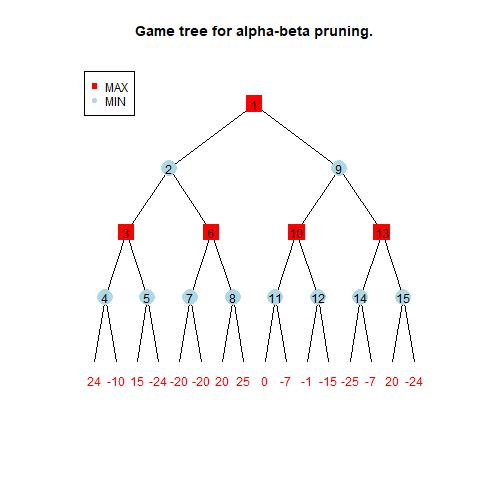
\includegraphics[width=\textwidth]{ab.jpg}
\end{figure}
\clearpage
\section{Scheduling}

Provide a complete resource constrained schedule for the actions found in Table~\ref{schActions}. (4 marks)
\begin{table}[h!]
\caption{Actions}
\label{schActions}
\begin{center}
\begin{tabular}{ |c|c|c|c|c|c| } 
\hline
 Index & Action & Duration & Uses & Consumes & After \\
\hline
1 & Start & 0 &   & 0 nails & NA\\
2 & Action 1 & 35 &  Saw & -1 nail & 1\\
3 & Action 2 & 45 &  Saw & 0 nails & 1\\
4 & Action 3 & 10 &   & -1 nail & 1\\
5 & Action 4 & 15 &   & 0 nails & 4\\
6 & Action 5 & 25 &   & 1 nail & 4,2,5\\
7 & Action 6 & 50 &  Saw & 0 nails & 3,5\\
8 & Action 7 & 40 &   & 1 nail & 3,2,4\\
9 & Finish & 0 &   & 0 nails & 6,7,8\\
\hline
\end{tabular}
\end{center}
\end{table}
\clearpage
\section{Multi-Armed Bandit Optimization}

Image we are testing click through rates on three different web layouts. At the current point, the Dirichlet (beta) distributions associated with each layout have the parameters in Table~\ref{MABO1}.\begin{table}[h!]
\caption{Dirichlet (Beta) Parameters for Layout}
\label{MABO1}
\begin{center}
\begin{tabular}{ |c|c|c| } 
\hline
 Layout & Parameter 1 & Parameter 2 \\
\hline
A &  11  &  4 \\
B &  8  &  3 \\
C &  10  &  6 \\
\hline
\end{tabular}
\end{center}
\end{table}

The first value is associated with not clicking through, the second clicking through.

A new person views the site. We generate samples from the distributions to determine which layout is used. These samples are given in Table~\ref{MABO2}.
\begin{table}[h!]
\caption{Samples from Layout Dirichlet (Beta) Distributions}
\label{MABO2}
\begin{center}
\begin{tabular}{ |c|c|c|c|c|c| } 
\hline
 Layout & Sample 1 & Sample 2 & Sample 3 & Sample 4 & Sample 5 \\
\hline
A &  0.25  &  0.15  &  0.31  &  0.29  &  0.39 \\
A &  0.25  &  0.14  &  0.22  &  0.26  &  0.26 \\
A &  0.2  &  0.19  &  0.32  &  0.48  &  0.18 \\
\hline
\end{tabular}
\end{center}
\end{table}


When shown the website with the chosen layout, the person makes a purchase ('clicks through'). Give the new parameters of the three distributions after this event. (2 Marks)
\clearpage
\section{Basic Feed-Forward ANNs}

Examine the neural network given in the diagram labelled 'Basic Regression Feed-Forward Neural Network'. In this diagram, square nodes represent biases, blue nodes the input layer, green nodes a hidden layer, and red nodes the output layer. The first round blue input node is associated with feature X1, and the second with feature X2 (counting downwards). Assuming that all activation functions are rectifiers (i.e. the hidden nodes are ReLU units), and the output is a basic linear regression function, calculate the output of this network if it was given an input of X1 = 5 and X2 = -5. Show all working. (2 Marks)

\begin{figure}[h!]
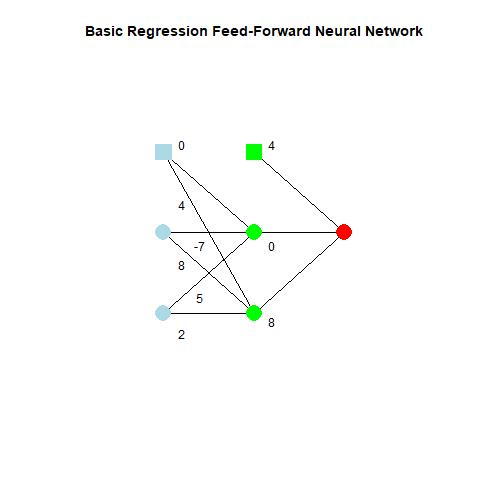
\includegraphics[width=\textwidth]{ffnn.jpg}
\end{figure}
\clearpage
\section{Convolution layers in CNNs}

Tables~\ref{CNN1} to~\ref{CNN3} provide an input matrix and two filter matrices for a convolutional layer in a CNN. Assuming no padding, that stride is [1,1], and that all activation functions are rectifiers, calculate the output of this layer. (2 marks)
\begin{table}[h!]
\caption{Input Matrix}
\label{CNN1}
\begin{center}
\begin{tabular}{ |c|c|c| } 
\hline
-3  &  -2  &  1 \\
-3  &  4  &  -3 \\
-2  &  -4  &  0 \\
\hline
\end{tabular}
\end{center}
\end{table}
\begin{table}[h!]
\caption{Filter 1}
\label{CNN2}
\begin{center}
\begin{tabular}{ |c|c| } 
\hline
4  &  -4 \\
1  &  2 \\
\hline
\end{tabular}
\end{center}
\end{table}
\begin{table}[h!]
\caption{Filter 1}
\label{CNN3}
\begin{center}
\begin{tabular}{ |c|c| } 
\hline
-2  &  -2 \\
3  &  -4 \\
\hline
\end{tabular}
\end{center}
\end{table}
\clearpage
\section{ Bias-Variance }

Give a basic explanation (as per what was discussed in the course) of the bias and variance components of expected error and their relationship to model complexity. (3 marks)
\clearpage
\section{ Reinforcement Learning }

What is the purpose of including randomness in the action-deciding process of a reinforcement learning system? (1 mark)\clearpage
\section{ LSTMs }

Explain the steps involving the memory vector in a pass through a LSTM layer at time t. Mention what is done to the memory vector (non-mathematically) and/or what the memory vector is used for in each of these steps. Make reference to the input at time t, and the outputs of time t-1 and t. (2 marks)\clearpage
\section{ Local Search }

Greedy Hill Climb suffers from the problem of local optima. Name and provide a brief explanation of three alternative local search strategies covered in this course that attempt to overcome or minimize this problem. (3 marks)
\clearpage
\section{ Planning Graphs }

Explain the two ways a planning graph can be used to provide a heuristic for A*. (2 marks)
\clearpage
\section{ Depth-First Search }

Under what conditions could a depth-first search FAIL to find a solution (in a finite search space with at most a single edge between any two nodes)? (1 mark)\clearpage
\section{ PDDL }

What is PDDL? Explain all components of a PDDL problem. Be as precise and concise as possible.  (4 marks)
\clearpage
\section{ Iterated Deepening }

Explain iterated deepening. (2 marks)
\clearpage
\section{ GANs }

Assume you have a GAN where the discriminator network is a simple binary (Genuine/Fake) classifier. Briefly explain how the generator network is trained. (2 marks)

\end{document}
